%%%%%%%%%%%%%%%%%%%%%%%%%%%%%%%%%%%%%%%%%%%%%%%%%%%%%%%%%%%%%%%%%%%%%%%%%%%%%%%%%%%%%%%%%%
\section{Discussion}

%%%%%%%%%%%%%%%%%%%%%%%%%%%%%%%%%%%%%%%%%%%%%
\subsection{Manual feature selection}

% sklearn random forest  

\begin{table}[H]
    \centering
    \caption{Ranking of feature importance from best to worst with respect to
    impurity decrease for three different reconstruction methods on the full
    dataset obtained with sci-kit learn.}  
    \label{tab:feature_importance}  

    \begin{tabular}{|c|c|c|c|}
        \hline
        Rank & Feature index & Feature name & Impurity decrease \\     
        \hline
        0       & 2           & histogram min  & 0.102915  \\
        1      & 12            & glcm entropy  & 0.088981  \\
        2      & 11           & glcm contrast  & 0.083777  \\
        3       & 4           & histogram std  & 0.081181  \\
        4      & 13        & glcm homogeneity  & 0.080463  \\
        5       & 5      & shape area\_density  & 0.073690  \\
        6       & 3          & histogram peak  & 0.069483  \\
        7       & 0           & histogram max  & 0.064857  \\
        8      & 14      & glcm joint\_maximum  & 0.061548  \\
        9       & 9    & shape volume\_density  & 0.055089  \\
        10      & 8            & shape volume  & 0.051088  \\
        11      & 7           & shape surface  & 0.048897  \\
        12     & 10            & glcm cluster  & 0.048494  \\
        13      & 1          & histogram mean  & 0.047758  \\
        14      & 6  & shape convex\_hull\_area  & 0.041778  \\
        \hline
         
    \end{tabular} 
\end{table}


% Identify features with poor class separation

% Identify highly correlated features  
% * plot correlation matrix  

\begin{figure}[H]
    \centering
    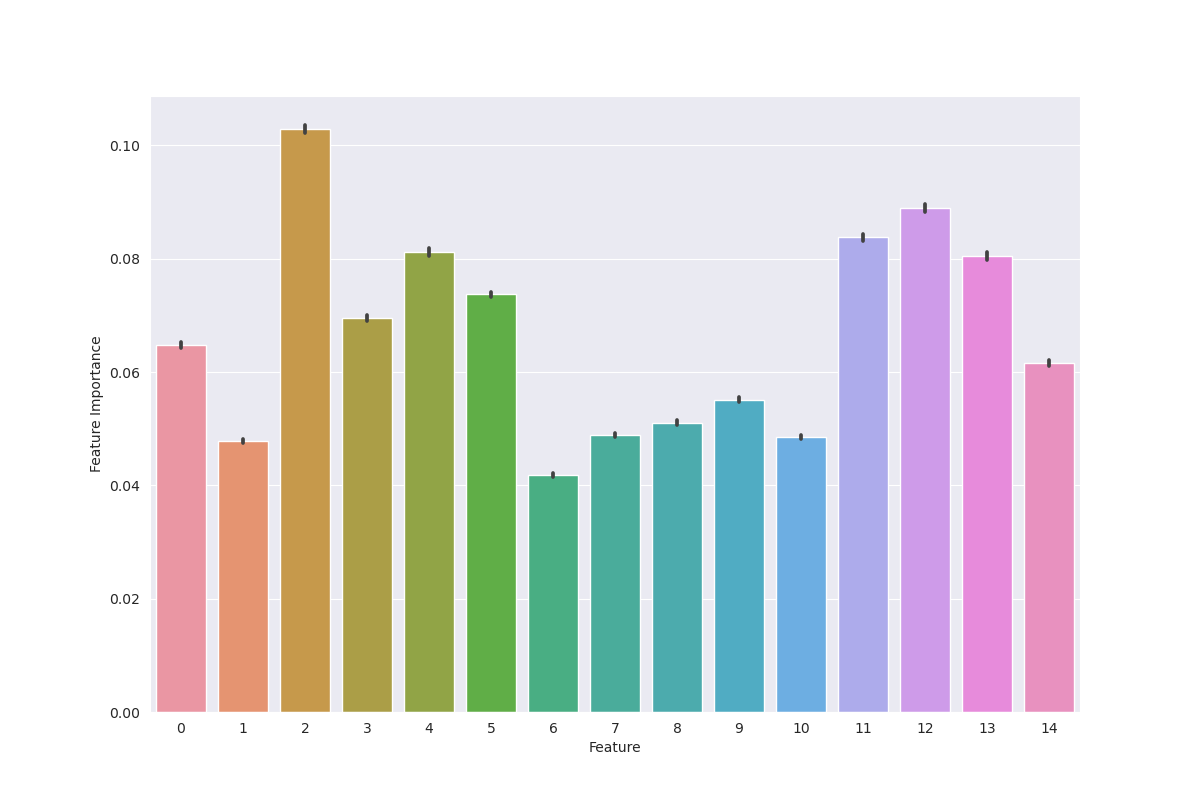
\includegraphics[width=0.8\textwidth]{Figures/feature_importance_sklearn_3s.png}
    \caption{Mean of the feautre\_importacnes\_ (purity decrease) for each decision tree. The
    error bar shows the 95\% confidence interval. The x-axis represent feature
    number as defined in table \ref{tab:feature_names}.  }  
    \label{fig:feature_importance} 
\end{figure}


\begin{figure}[H]
    \centering
    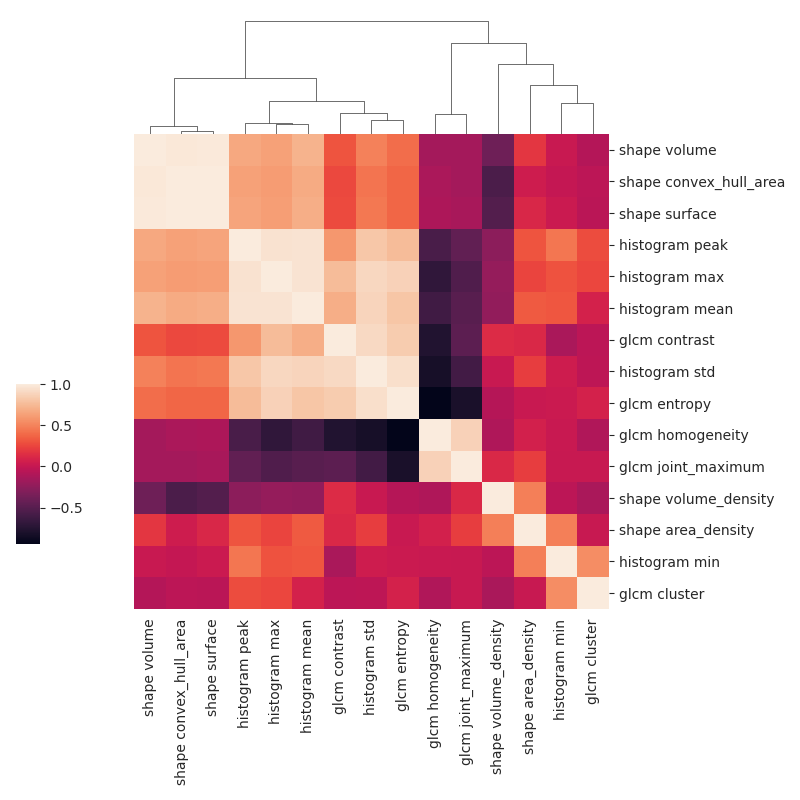
\includegraphics[width=1\textwidth]{Figures/feature_correlation.png}
    \caption{Pearson Correlation between each feature calculated on the full
    dataset. }  
\end{figure}





%%%%%%%%%%%%%%%%%%%%%%%%%%%%%%%%%%%%%%%%%%%%%
\subsection{Compare Manual VS Automatic feature reduction}
\begin{itemize}
    \item Is the Automatic selection method as expected, compared with visual
        inspection, manual feature reduction.   
\end{itemize}





